\documentclass[12pt]{article}
\usepackage[a4paper, total={6in, 8in}]{geometry}
\usepackage[utf8]{inputenc}
\usepackage{tikz,pgfplots}
\usetikzlibrary{positioning}
\usetikzlibrary{datavisualization}
\usetikzlibrary {datavisualization.formats.functions}
\usepackage{fontenc}
\usepackage{amssymb}
\usepackage{mathrsfs}
\usepackage{amsmath}
\usepackage{graphicx}
\usepackage{subcaption}
\usepackage{setspace}
\singlespacing




\title{\emph{Chapter1:The Physics of Waves}}
\author{Yijie Chen}
\date{}


\numberwithin{equation}{section}
\begin{document}
\maketitle
\tableofcontents
\newpage
\section{One-dim wave equation}
    \indent All classical mechanical waves can be described by the same equation,the \emph{differential wave equation:}
    \begin{equation}
        \frac{\partial^2{\Psi(x,t)}}{\partial{x^2}}=\frac{1}{v^2}\frac{\partial^2{\Psi(x,t)}}{\partial{t^2}}\label{11}
    \end{equation}
\subsection{Example}
    Show that
    \\
    \[\Psi(x,t)=(x+vt)^2\]
    \\
    is a solution to the differential wave equation.Assume that $v$ is a constant.\\
    \indent \textbf{Solution}\\
    \indent  We must show that $\Psi(x,t)$ solves Equation \eqref{11}:
    \[
    \frac{\partial^2{\Psi(x,t)}}{\partial{x^2}}=\frac{1}{v^2}\frac{\partial^2{\Psi(x,t)}}{\partial{t^2}}
    \]
    \indent To do this,we must take the indicated derivatives.Begin with the partial derivative with respect to $x$:
    \[
    \frac{\partial{\Psi(x,t)}}{\partial{x}}=\frac{\partial}{\partial{x}}(x+vt)^2=2(x+vt)\frac{\partial}{\partial{x}}(x+vt)=2(x+vt)(1)=2(x+vt)
    \]
    \indent Now take the second partial derivative with respect to $x$:
    \[
    \frac{\partial^2{\Psi}}{\partial{x^2}}=\frac{\partial}{\partial{x}}[\frac{\partial{\Psi}}{\partial{x}}]=\frac{\partial}{\partial{x}}[2(x+vt)]=2
    \]
    \indent Next,take the partial derivatives of $\Psi(x,t)$ with respect to $t$:
    \[
    \frac{\partial{\Psi}}{\partial{t}}=2(x+vt)\frac{\partial}{\partial{t}}(x+vt)=2(x+vt)(v)=2v(x+vt)
    \]
    \[
    \frac{\partial^2{\Psi}}{\partial{t^2}}=\frac{\partial}{\partial{t}}[2v(x+vt)]=\frac{\partial}{\partial{t}}[2vx+2v^2t]=2v^2
    \]
    \indent Substitute these results into the differential wave equation.
    \[
    \frac{\partial^2{\Psi(x,t)}}{\partial{x^2}}=2
    \]
    \[
    \frac{1}{v^2}\frac{\partial^2{\Psi(x,t)}}{\partial{t^2}}=\frac{1}{v^2}(2v^2)=2
    \]
    \indent Thus
    \[
    \frac{\partial^2{\Psi(x,t)}}{\partial{x^2}}=\frac{1}{v^2}\frac{\partial^2{\Psi(x,t)}}{\partial{t^2}}
    \]
    \indent $\Psi(x,t)$ solves the differential wave equation,and thus we have shown that it is a traveling wave.

\section{General solutions to the one-dim wave equation}
    We will show below that the most general solutions to Equation\eqref{11} may be expressed as follows:
    \begin{equation}
        \Psi(x,t)=f(x-vt)\label{21}
    \end{equation}
    \begin{equation}
        \Psi(x,t)=g(x+vt)\label{22}
    \end{equation}
    \indent where the function $f$ and $g$ represent any function that has finite second derivatives,and where 
    the parameters $x$,$v$ and $t$ all occur explicitly within the function as $x-vt$ or $x+vt$.\\
    \indent As an example,consider the function
    \begin{equation}
        \Psi(x,t)=\frac{A}{1+(x-vt)^2}\label{23}
    \end{equation}
    \indent where $A$ is a constant.Equation\eqref{23} represents a peaked function whose maximum is located at points given by $x=vt$. A plot of this wave function at two different times is shown in Figure \ref{f1}.\\
    \begin{figure}[h]
        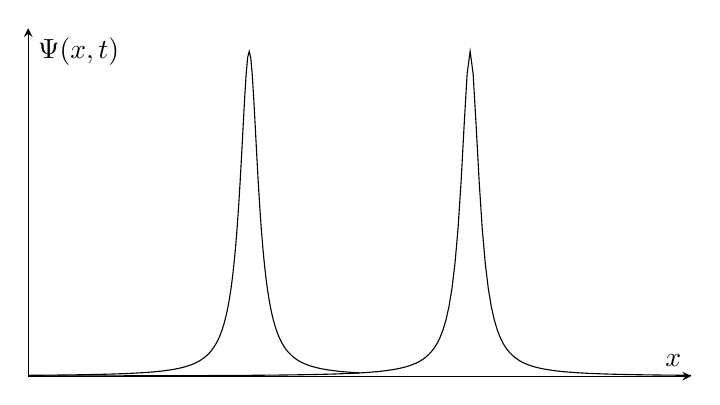
\begin{tikzpicture}
            \begin{axis}[
              width=10cm,
              height=6cm,
              axis lines=middle,
              xmin=0, xmax=60,
              ymin=0, ymax=30,
              ticks=none, % removes ticks
              legend style={draw=none},
              xlabel={$x$}, % removes x-axis label
              ylabel={$\Psi(x,t)$}, % removes y-axis label
            ]
            % Plot the function
            \addplot[black, domain=0:30, samples=220] {28/(1+(x-20)^2)};
            \addplot[black, domain=0:60, samples=220] {28/(1+(x-40)^2)};
            \end{axis}
        \end{tikzpicture}
        \centering
        \caption{The traveling pulse of Equation \eqref{23}, shown at two different times $t_1<t_2$.}
        \label{f1}
    \end{figure}
    \newpage
    \indent Velocity $v$ is determined,$x$ depends on time $t$. While $vt_1=x$ or $vt_2=x$, $\Psi(x,t)=A$ , $x$ is a coordinates of wave occurs pulse during traveling.\\
    \indent While $v$ has a plus sign,such as $+v$,we have $x-(+v)t=x-vt$ in Equation\eqref{21},wave \emph{traveling forward} and $v$ has a minus sign, such as $-v$,$x-(-v)t=x+vt$ in Equation\eqref{22},\emph{wave traveling backward}.
\subsection{Example}
    Show that\\
    \[
    \Psi(x,t)=Ae^{-(a^2x^2+b^2t^2+2abxt)}
    \]
    is a traveling wave,and find the wave speed and direction of propagation.Assume that $A$,$a$ and $b$ are all constants,and that $a$ and $b$ have units that make the quantity in the exponential function unitless.\\
    \indent \textbf{Solution}\\
    \[
    \Psi(x,t)=Ae^{-(a^2x^2+b^2t^2+2abxt)}
    \]
    \[
    =Ae^{-(ax+bt)^2}
    \]
    \indent While $ax+bt=0$, thus $x=-\frac{bt}{a}$ and $v=-\frac{b}{a}$,this wave traveling backward.
\section{Harmonic traveling waves}
    According to the results of the previous section,any function described by Equation\eqref{21} or \eqref{22} represents a 
    traveling wave. In particular,\emph{harmonic function}(i.e.,sines and consines) with the appropriate arguments solve the differential wave equation.Thus,the following function represents a traveling wave:
    \\
    \begin{equation}
        \Psi(x,t)=Asin\frac{2\pi}{\lambda}(x\mp vt)\label{31}
    \end{equation}
    The $\Psi(x,t)$ given in Equation\eqref{31} is periodic in both space and time coordinates.The term $\lambda$ represents the \emph{spatial period}:
    \[
    \Psi(x+\lambda ,t)=Asin\frac{2\pi}{\lambda}(x+\lambda \mp vt)=Asin[\frac{2\pi}{\lambda}(x\mp vt)+2\pi]=\Psi(x,t) 
    \]
    Let T represent the \emph{temporal period};the time required for one cycle.Since Equation\eqref{31} is periodic in T,we have
    \[
    \Psi(x,t+T)=Asin\frac{2\pi}{\lambda}[x\mp v(t+T)]=Asin[\frac{2\pi}{\lambda}(x\mp vt)\mp \frac{2\pi}{\lambda}vT]
    \]
    T represents the temporal period provided that
    \\
    \begin{equation}
        \frac{vT}{\lambda}=1\label{32}
    \end{equation}
    \\
    or 
    \\
    \begin{equation}
        v=\frac{\lambda}{T}\label{33}
    \end{equation}
    \\
    Thus,a periodic classical wave travels one wavelength $\lambda$ in one temporal period T.It is customary to define the wave\emph{frequency} as 
    \\
    \begin{equation}
        f=\frac{1}{T}\label{34}
    \end{equation}
    \\
    In terms of frequency,\eqref{33} becomes
    \begin{equation}
        f\lambda=v\label{35}
    \end{equation}
    \\
    A plot of $\Psi(x,t)$ vs. $x$ is shown in Figure \ref{f2a}. Figure \ref{f2b} shows a plot of $\Psi(x,t)$ vs. $t$.\\
    It is customary to define the \emph{propagation constant} as follows:
    \begin{equation}
        k=\frac{2\pi}{\lambda}\label{36}
    \end{equation}
    This quantity is also sometimes referred to as the \emph{wave number}.Since k converts meters to radians,the units are r $ad/m$.We may rewrite Equation \eqref{31} as 
    \[
        \Psi(x,t)=Asink(x\mp vt)
    \]
    \newpage
    \begin{figure}[h]
        \centering
        \begin{subfigure}[b]{0.45\textwidth}
            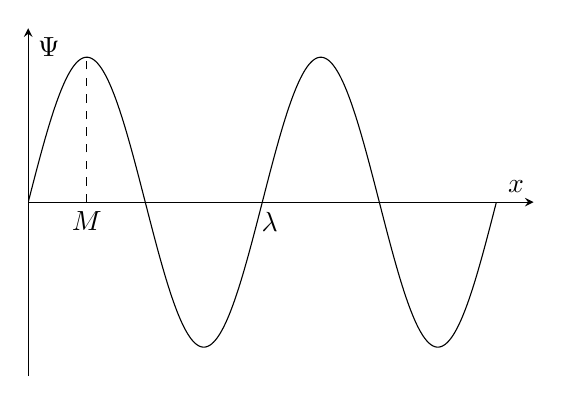
\begin{tikzpicture}
                \begin{axis}[
                    width=8cm,
                    height=6cm,
                    axis lines=middle,
                    xmin=0, xmax=4*pi+1,
                    ymin=-1.2, ymax=1.2,
                    ticks=none, % removes ticks
                    legend style={draw=none},
                    xlabel={$x$}, % removes x-axis label
                    ylabel={$\Psi$}, % removes y-axis label
                ]
                \draw[dashed] (axis cs:pi/2,0) -- (axis cs:pi/2,1);
                \addplot[black,domain=0:4*pi,samples=400] {sin{deg(x)}};
                \node[below] at (axis cs:pi/2,0) {$M$};
                \node[below] at (axis cs:2*pi+0.2,0) {$\lambda$};
                \end{axis}
                
              \end{tikzpicture}
            \caption{}
          \label{f2a}
        \end{subfigure}
        \hfill
        \begin{subfigure}[b]{0.45\textwidth}
            \begin{tikzpicture}
                \begin{axis}[
                    width=8cm,
                    height=6cm,
                    axis lines=middle,
                    xmin=0, xmax=4*pi+1,
                    ymin=-1.2, ymax=1.2,
                    ticks=none, % removes ticks
                    legend style={draw=none},
                    xlabel={$t$}, % removes x-axis label
                    ylabel={$\Psi$}, % removes y-axis label
                ]
                \addplot[black,domain=0:4*pi,samples=400] {cos{deg(x)}};
                \node[below] at (axis cs:3*pi/2+0.3,0) {$T$};
                \end{axis}
              \end{tikzpicture}
              \caption{}
          \label{f2b}
        \end{subfigure}
      
        \caption{Plots of harmonic wavefunction. (a) A plot of $\Psi(x,t)$ vs. position $x$. (b)
        A plot of $\Psi(x,t)$ vs. time using data recorded by a single measuring device located at $M$ in Figure (a)}
        \label{f2}
      \end{figure}
    Similarly, we can define the \emph{angular frequency} 
    \begin{equation}
        \omega=kv=\frac{2\pi}{\lambda}v=2\pi f\label{37}
    \end{equation}
    Since $\omega$ converts time to radians,the units are r $ad/s$. Note that according to the last result.
    \begin{equation}
        \frac{\omega}{k}=v\label{38}
    \end{equation}
    \indent In terms of k and $\omega$, Equation \eqref{31} becomes
    \[
        \Psi(x,t)=Asin(kx\mp \omega t)
    \]
    Collectively, the terms $kx \mp\omega t$ are called the \emph{phase} of the harmonic traveling wave. We may also include an explicit value of the phase when x and t are zero by specifying the \emph{initial phase} $\phi$:
    \begin{equation}
        \Psi(x,t)=Asin(kx\mp \omega t+\phi)\label{39}
    \end{equation}
\subsection{Example}
A harmonic traveling wave is given by $\Psi(z,t)=Asin(50z+3000t)$.Find the wave speed,frequency,angular frequency,and direction of propagation.
\\
\indent \textbf{Solution}
\[
    \Psi(z,t)=Asin(50z+3000t)=Asin(kz+\omega t)
\]
\[
    k=\frac{2\pi}{\lambda}=50
\]
\[
    \omega=kv=2\pi f=3000
\]
wave speed:
\[
    v=\frac{3000}{k}=60
\]
frequency:
\[
    f=\frac{3000}{2\pi}=\frac{1500}{\pi}
\]
angular frequency:
\[
    \omega=3000
\]
direction of propagation:backward 
\section{The three-dimensional wave equation}
In Cartesian coordinates,the extension of Equation \eqref{11} to include three dimensions is made in the obvious way:
\begin{equation}
    \frac{\partial^2 {\Psi}}{\partial{x^2}}+\frac{\partial^2 {\Psi}}{\partial{y^2}}+\frac{\partial^2 {\Psi}}{\partial{z^2}}=\frac{1}{v^2}\frac{\partial^2 {\Psi}}{\partial{t^2}}\label{41}
\end{equation}
where $\Psi=\Psi(x,y,z,t)$ is now understood to be a function of time and all three spatial coordinates.\\
\indent Equation\eqref{41} can be written in a more general form using the Laplacian operator:
\begin{equation}
    \nabla^2{\Psi}=\frac{1}{v^2}\frac{\partial^2{\Psi}}{\partial{t^2}}\label{42}
\end{equation}
\\
where in Cartesian coordinates,the \emph{Laplacian} is given by
\begin{equation}
    \nabla^2=\frac{\partial^2 }{\partial{x^2}}+\frac{\partial^2 }{\partial{y^2}}+\frac{\partial^2 }{\partial{z^2}}\label{43}
\end{equation}
Equation \eqref{42} is the \emph{coordinates independent} representation of the three-dimensional wave equation.
\subsection{Three-Dimensional Plane Waves}
Consider an acoustic wave traveling through air.In a three-dimensional \emph{plane wave},the
properties of the medium are constant over any \emph{plane} oriented normal to the direction of propagation.
To describe such a wave,we define the propagation vector $\vec{k}$ with magnitude $\frac{2\pi}{\lambda}$ and direction given by the wave propagation.The corresponding plane wave is given by
\begin{equation}
    \Psi(x,y,z,t)=Asin(\vec{k}\cdot \vec{r}-\omega t+\varphi)\label{44}
\end{equation}
A plane has Cartesian symmetry,and in Cartesian coordinates,$\vec{k}$ is given by
\begin{equation}
    \vec{k}=k_x\hat{i}+k_y\hat{j}+k_z\hat{k}\label{45}
\end{equation}
The position vector in Cartesian coordinates is given by 
\begin{equation}
    \vec{r}=x\hat{i}+y\hat{j}+z\hat{k}\label{46}    
\end{equation}
For example, in a plane harmonic sound wave traveling in the positive \emph{x}-direction,the value of the air pressure is constant over any plane that is parallel to the \emph{y-z} plane:
\begin{equation}
    \Psi(x,y,z,t)=Asin(kx-\omega t+\varphi)\label{47}
\end{equation}
\indent In Figure it is seen that $\vec{k}$ is normal to planes defined by $\vec{k}\cdot\vec{r}=\emph{const}$.It is convenient to 
define \emph{wavefronts} located at points where the phase of Equation \eqref{44} is equal to integer multiples of $2\pi$.
Thus,a three-dimensional plane wave may be visualized as a train of wavefronts separated by one wavelength $\lambda$ and moving with the wave speed v.\\
\indent In the complex representation,harmonic plane waves are given by
\begin{equation}
    \Psi(x,y,z,t)=Ae^{i(\vec{k}\cdot\vec{r}-\omega t+\varphi)}\label{48}
\end{equation}
\subsection{Spherical Waves}
\emph{Spherical waves} are waves with wavefronts that are spherical in shape. Examples include waves that emanate from an isotropic point source,or are converging to a point.
An isotropic source emits waves symmetrically in all directions.\\
\indent In spherical coordinates,spherical waves have no dependence on the angular coordinates $\theta$ and $\phi$,so the derivatives with respect to these coordinates are zero,this means that the
\[
    \Psi(\vec{r},t)=\Psi(r,t)
\]
In otherwords,$\Psi(r,t)$ depends only on the spherical coordinates $r$ and time t.Derivatives of such a function with respect to $\theta$ and $\phi$ given zero,leading to a simplified version of the Laplacian for spherical coordinates:
\begin{equation}
    \nabla^2=\frac{1}{r^2}\frac{\partial}{\partial{r}}(r^2\frac{\partial}{\partial{r}})\label{49}
\end{equation}
Using this Laplacian, we obtain the \emph{spherical symmetric differential wave equation}:
\begin{equation}
    \frac{1}{r^2}\frac{\partial}{\partial{r}}(r^2\frac{\partial{\Psi(r,t)}}{\partial{r}})=\frac{1}{v^2}\frac{\partial^2{\Psi(r,t)}}{\partial{t^2}}\label{410}
\end{equation}
An important solution to this equation is the \emph{harmonic spherical wave}
\begin{equation}
    \Psi(r,t)=\frac{A}{r}sin(kr \mp \omega t+\varphi)\label{411}
\end{equation}
If the minus sign is chosen,the wave emanate from an isotropic source located at $r=0$.
A plus sign represents a wave that is converging to the point $r=0$.The amplitude $\frac{A}{r}$ of 
the wave is not constant,since it depends on radial coordinate $r$.For a wave emanating from a point,
the amplitude decreases as the wave travels. Waves converging to a point have amplitudes that increase as time increases.\\
\indent  In the complex representation,Equation \eqref{411} becomes
\begin{equation}
    \Psi(r,t)=\frac{A}{r}e^{i(kr \mp \omega t+\varphi)}
\end{equation}
\newpage
\appendix
\section{Appendix:Complex Numbers and the Complex Representation}
\emph{Complex} numbers can provide algebraic shortcuts that will prove very convenient as we continue our discussion of classical optics.
In this section,we provide a quick overview of the properties of complex numbers,and a few of their algebraic features that we will find most useful.\\
\indent Complex numbers include the concept of the \emph{imaginary number $i$}:
\begin{equation}
    i=\sqrt{-1}
\end{equation}
Clearly,the square root of a negative number has no counterpart within the set of all \emph{real} numbers.A complex number $z$ has both a real part and an imaginary part:
\begin{equation}
    z=x+iy
\end{equation}
where x is the \emph{real} part of z and y is the \emph{imaginary} part of z.\\
\indent In the \emph{Cartesian representation}, a complex number is plotted with coordinates (x,y);
thus the horizontal axis is called the \emph{real axis}, and the vertical axis is called \emph{imaginary axis}.\\
\indent Many of the features of complex numbers that we will find most useful result from the \emph{Euler relation}:
\begin{equation}
    e^{i\theta}=cos \theta+isin \theta\label{53}
\end{equation}
We may use the Euler relation to express any complex number z in polar form.Let
\begin{equation}
    x=r cos \theta
\end{equation}
\begin{equation}
    y=r sin \theta
\end{equation}
\begin{figure}
    \centering
    \begin{tikzpicture}
        \begin{axis}[
            axis lines=middle,
            width=8cm,
            height=8cm,
            xmin=-7,xmax=7,
            ymin=-7,ymax=7,
            ticks=none,
            xlabel={$Re$},
            ylabel={$Im$},
            legend style={draw=none},   
        ]
        \draw [solid] (axis cs:0,0) -- (axis cs:0,7);
        \draw [solid] (axis cs:0,0) -- (axis cs:0,-7);
        \draw [solid] (axis cs:0,0) -- (axis cs:-7,0);
        \draw [solid] (axis cs:0,0) -- (axis cs:7,0);
        \draw [->,thick] (axis cs:0,0) -- (axis cs:5,5);
        \node[below] at (axis cs:1.5,1.2) {$\theta$};
        \node[below] at (axis cs:2,3.5) {$r$};
        \node[below] at (axis cs:5.5,6.5) {$(x,y)$};
        \end{axis}
    \end{tikzpicture}
    \caption{The comple plane}
\end{figure}
\newpage
where
\begin{equation}
    r=\sqrt{x^2+y^2}\label{56}
\end{equation}
\begin{equation}
    \theta=tan^{-1}({\frac{y}{x}})
\end{equation}
Using these relation,we may represent $z$ as
\begin{equation}
    z=x+iy=rcos \theta+i(rsin \theta)
\end{equation}
Thus,according to Equation \eqref{53},
\begin{equation}
    z=re^{i\theta}
\end{equation}
In thr polar representation,r is called the \emph{magnitude} of z,and $\theta$ is called the \emph{phase} of z.\\
The following examples are often useful:\\
\begin{equation}
    e^{\pm i(2\pi)}=1;e^{\pm i(\pi)}=-1;e^{i\frac{\pi}{2}}=i;e^{i\frac{3\pi}{2}}=-i
\end{equation}
\indent The \emph{complex conjugate $z^*$} of a complex number is z is obtained ny inverting the sign on each occurrence of i.For example, in the Cartesian representation where $z=x+iy$,$z^*$ is given by
\begin{equation}
    z^*=x-iy
\end{equation}
In the polar representation where $z=re^{i\theta}$, $z^*$ is given by
\begin{equation}
    z^*=re^{-i\theta}
\end{equation}
\indent Let $Re[z]$ and $Im[z]$ denote the real and imaginary parts of z. In the Cartesian form,Re[z]=x and Im[z]=y.
In the polar form,$Re[z]=rcos\theta$ and $Im[z]=rsin\theta$.In either case,
\begin{equation}
    Re[z]=\frac{z+z^*}{2}
\end{equation}
\begin{equation}
    Im[z]=\frac{z-z^*}{2i}
\end{equation}
According to the Euler relation,
\begin{equation}
    cos \theta=\frac{e^{i\theta}+e^{-i\theta}}{2}
\end{equation}
\begin{equation}
    sin \theta=\frac{e^{i\theta}-e^{-i\theta}}{2i}
\end{equation}
Multiplication of a complex number by its complex conjugate gives the square of the magnitude.In the Cartesian form,
\begin{equation}
    zz^*=(x+iy)(x-iy)=x^2+y^2
\end{equation}
and in the polar form,
\begin{equation}
    zz^*=(re^{i\theta})(re^{-i\theta})=r^2
\end{equation}
which,according to Equation \eqref{56},agrees with the previous result.We will also refer to the magnitude of $z$ as $\vert z \vert$:
\begin{equation}
    zz^*=\vert z \vert^2
\end{equation}




    


\end{document}



